\documentclass[fleqn]{llncs}
\usepackage[bottom]{footmisc}
\usepackage{graphicx}
\usepackage{cite}
\usepackage{caption}
\usepackage{subcaption}
\captionsetup{compatibility=false}
%\usepackage{amsbsy}
\usepackage[fleqn]{amsmath}
\usepackage{booktabs}
\usepackage{breqn}
\usepackage{tikz}
\usetikzlibrary{arrows}
\usepackage{lipsum}
\usepackage[affil-it]{authblk}
\usepackage[utf8]{inputenc}
\usepackage[english]{babel}
\interdisplaylinepenalty=2500
\pagenumbering{arabic}
\usepackage{array}
\usepackage[toc,page]{appendix}
\usepackage{bibnames}
\newcolumntype{R}[1]{>{\raggedleft\let\newline\\\arraybackslash\hspace{0pt}}m{#1}}


\title{Project 1 on PCA and Apriori Algorithm}
\begin{document}
	\author{Dong Xuanyu \and Yifu Yin \and Tiehang Duan}
	\institute{Department of Computer Science and Engineering\\The State University of New York at Buffalo\\Buffalo, NY 14260, United States\\
    \email{xuanyudo@buffalo.edu, yifuyin@buffalo.edu, tiehangd@buffalo.edu}}
	%\keywords{}
	\setcounter{page}{1}
	\maketitle
	\thispagestyle{plain}
	\pagestyle{plain}


	\begin{abstract}
	This project includes two interesting implementations, one on PCA dimensionality reduction algorithm and the other on Apriori algorithm. PCA serves the purpose of dimensionality reduction, and helps data visualization when the dimensionality is reduced to 2, and is mainly used in the field of computer vision to reconstruct images, while Apriori algorithms is widely used in database systems to infer useful rules out of transactions. In this project, we illustrate on the implementation details and also demonstrate our experiment results. \textbf{Our team made two different original implementations for each of these algorithms, as can be seen on our team's Github page: \url{https://github.com/xuanyudo/Pca_Apriori-Algorithm}.}
	
	 
	\end{abstract}

\section{Model Description}

\subsection{Principle Component Analysis} Principle component analysis is built on linear algebra. It can represent data in a more compact form by (1): get the covariance matrix of the dataset, (2): decompose the covariate matrix into a set of eigen vectors and eigen values, (3) pick out the {eigen value, eigen vector} pairs with the top k largest eigen value, if we want to visualize the data, then k will be set to 2 or 3. (4) The new set of coordinates for each of the data in the dataset will be the multiplication of original coordinates with each of the k eigen vectors, with each data point having k coordinates.


\subsection{Apriori Algorithm} The Apriori algorithm mines the association rules out of a frequent set given a set of transactions. The algorithm contains two steps: (1) generate a set of frequent items which exceeds the required support threshold, and (2) generate rules based on the frequent item sets which satisfies the confidence threshold. Direct computation of the frequent item sets and rules is infeasible given the exponential nature of the possible combinations, and further improvements including pruning technique to reduce the number of candidates, vertical based mining algorithms to reduce the number of transactions, and efficient data structures (hash tables) to reduce the number of comparisons is introduced in the field.




\section{Model Implementation} 

\subsection{Implementation of PCA} In this implementation, we encapsulated the whole functionality of PCA algorithm into one "PCA" class. After reading in the file and parse the dataset into a data matrix, the "compute covariant" function computes the covariance of the data matrix, whose dimensionality is of size $feature\ No. \times feature\ No.$. Then we called the "np.linalg.eig" function to calculate the eigen value and eigen vector of this covariance matrix, after which the two {eigen value, eigen vector} pairs with the largest eigen value is kept and serves as the new axises for the plot. Then, we get the coordinates of the each of the data point under this new set of coordinates, which is done by getting the inner product of the data point with each of the 2 eigen vectors. For the plot, we used a dictionary to store all the available colors which matches with the category that each data point belongs to.


\subsection{Application of TSNE Method} Based on the project guidance, we adopted readily available packages from sklearn.manifold for creation of the tsne plot. In the package, we call the TSNE function and set the parameter n\_components to be 2, so as it can be plotted as a two dimension scatter graph, and the data matrix is feed into the fit\_transform method. 


\subsection{Application of SVD Method} Based on the project guidance, we adopted readily available packages from np.linalg.svd for creation of the SVD plot. We attached visualization of the result below. 



\subsection{Implementation of Apriori Algorithm} 







\section{Experiment Result} 

\subsection{Result on PCA Analysis} After running PCA algorithm on the three given data files (pca\_a.txt, pca\_b.txt, pca\_c.txt), we plot the result in Figure \ref{fig2}. 





\begin{figure}
	\centering
	\begin{subfigure}{1.0\textwidth}
		\centering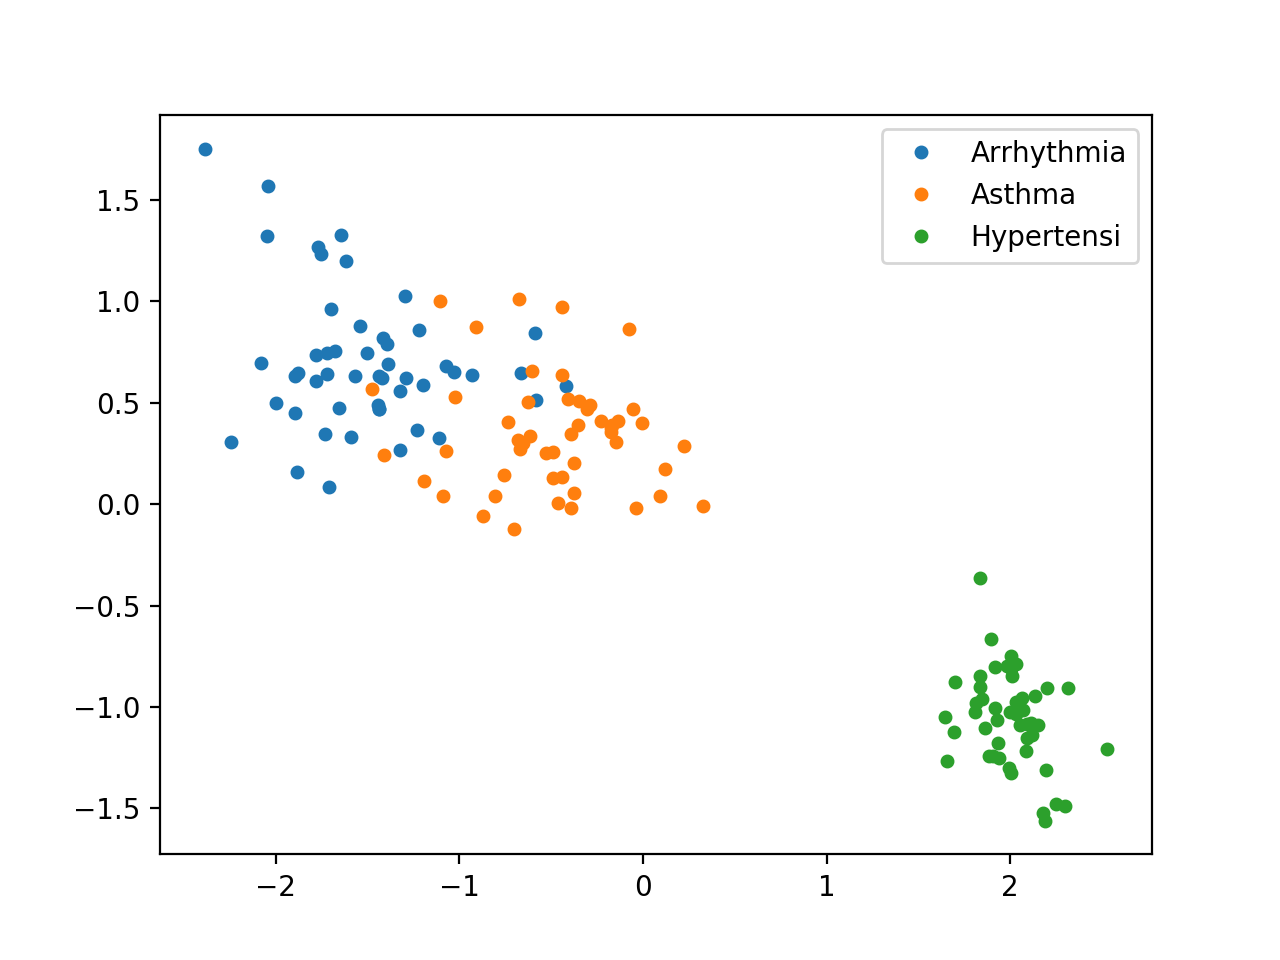
\includegraphics[width=0.7\textwidth]{pcaa_cal.png}
		\caption{PCA visualization of pca\_a.txt data file}
	\end{subfigure}
	\begin{subfigure}{1.0\textwidth}
		\centering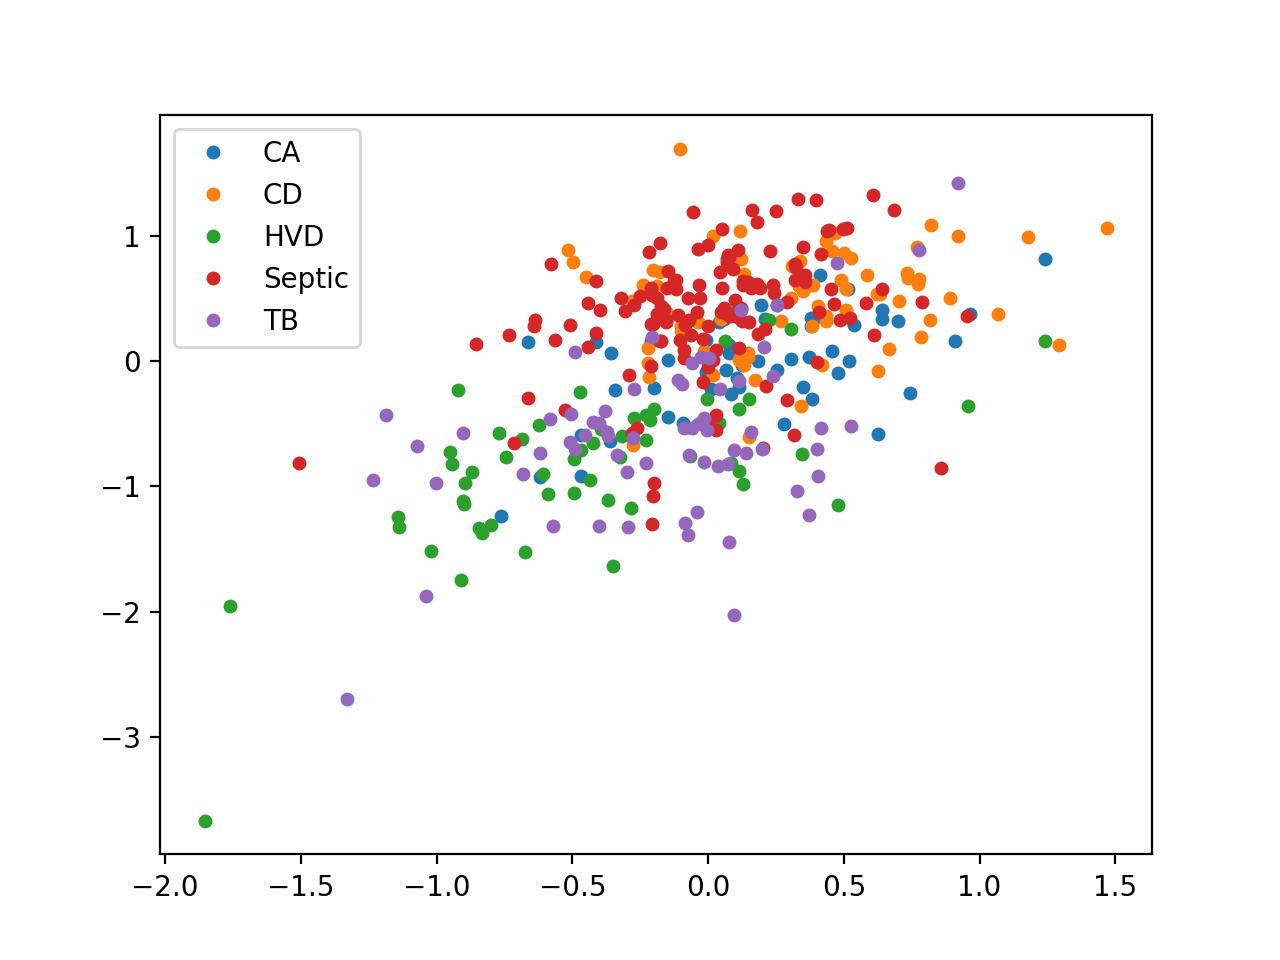
\includegraphics[width=0.7\textwidth]{pcab_cal.png}
		\caption{PCA visualization of pca\_b.txt data file}
	\end{subfigure}
	\begin{subfigure}{1.0\textwidth}
		\centering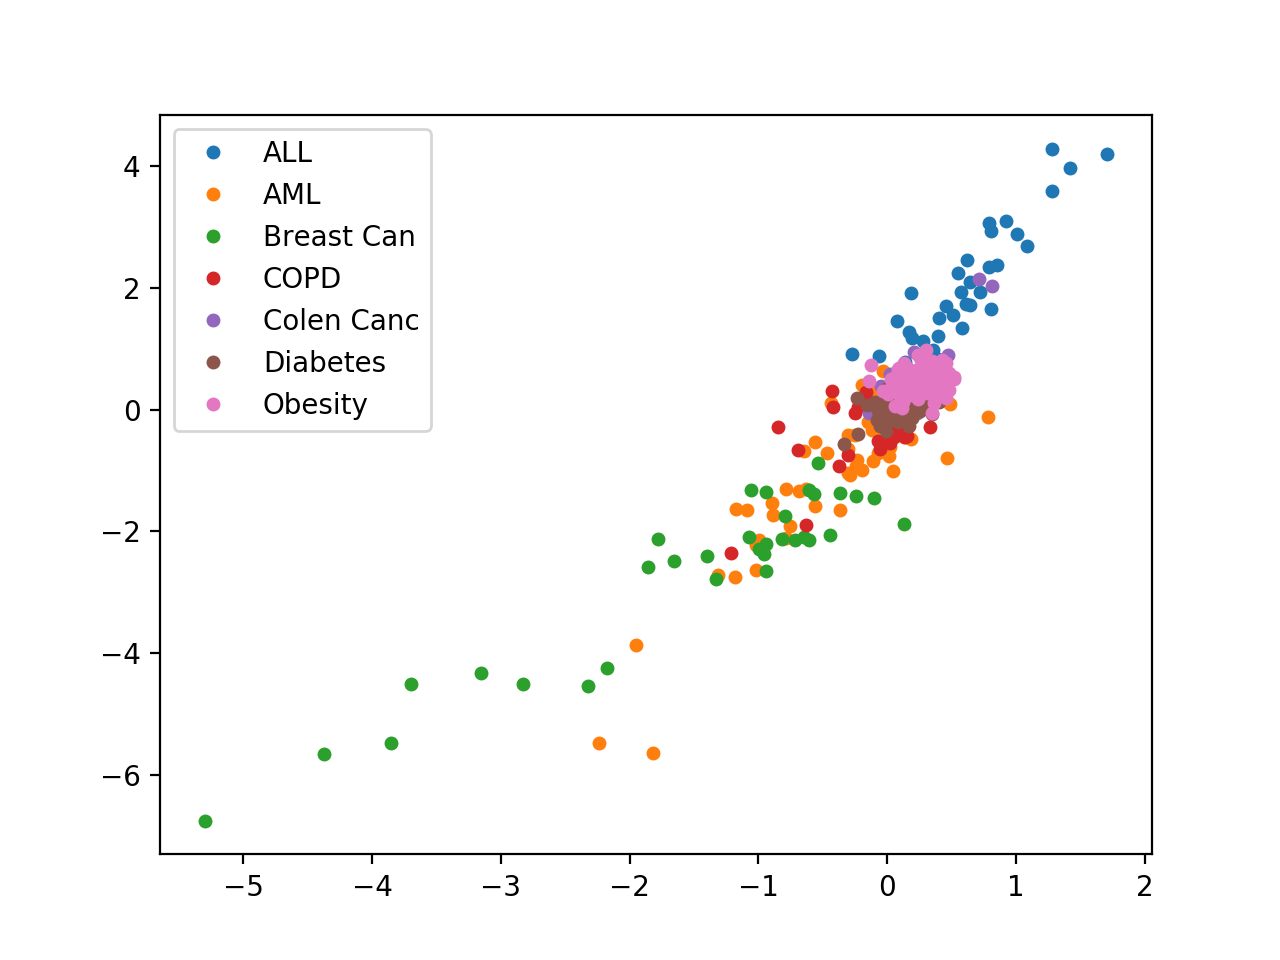
\includegraphics[width=0.7\textwidth]{pcac_cal.png}
		\caption{PCA visualization of pca\_c.txt data file}
	\end{subfigure}
	\caption{(a) PCA visualization of pca\_a.txt data file, (b) PCA visualization of pca\_b.txt data file, (c) PCA visualization of pca\_c.txt data file.}
	\label{fig2}
\end{figure}





\begin{figure}
	\centering
	\begin{subfigure}{1.0\textwidth}
		\centering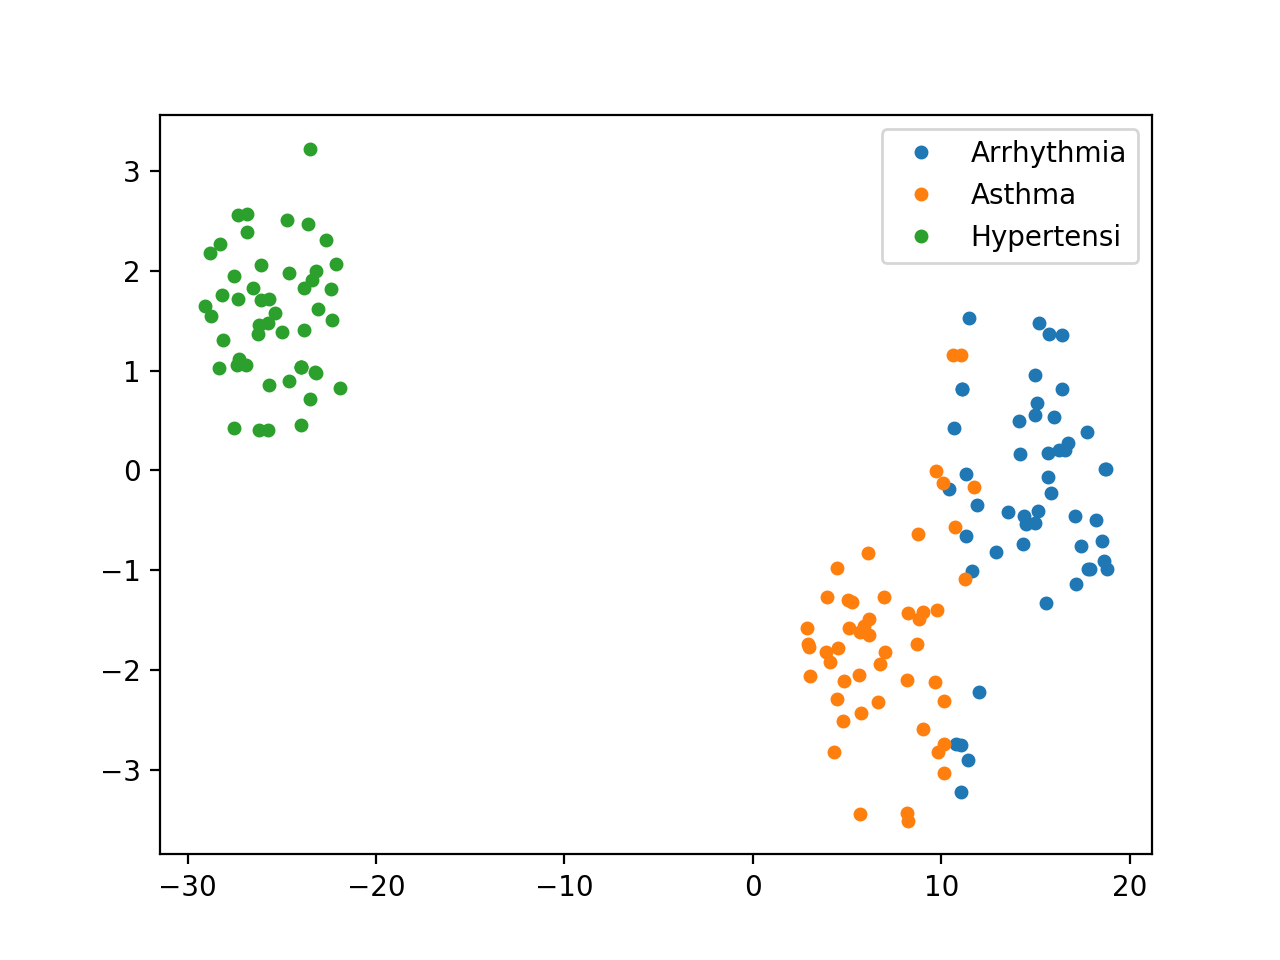
\includegraphics[width=0.7\textwidth]{tsnea.png}
		\caption{TSNE visualization of pca\_a.txt data file}
	\end{subfigure}
	\begin{subfigure}{1.0\textwidth}
		\centering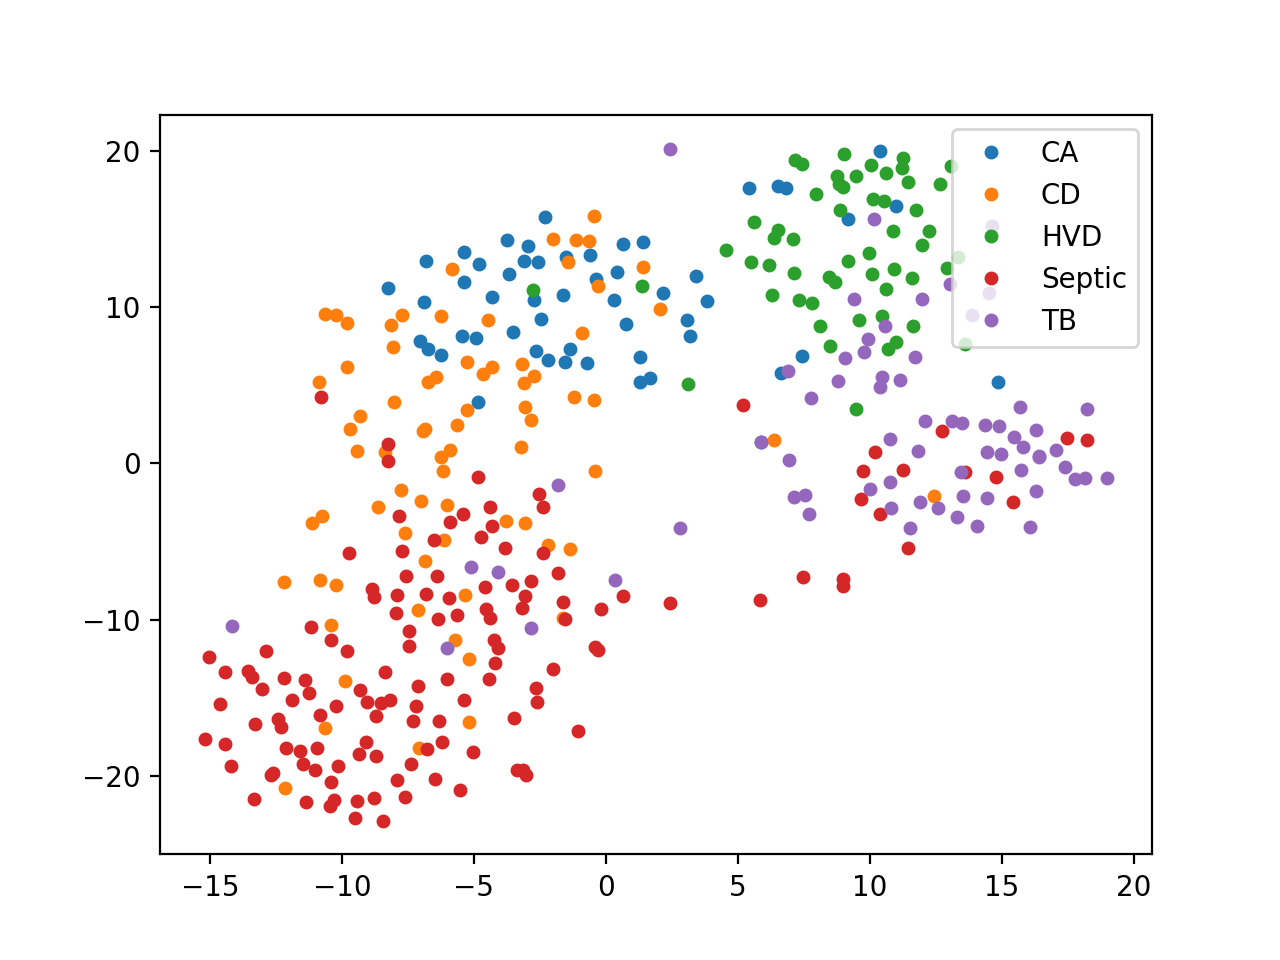
\includegraphics[width=0.7\textwidth]{tsneb.png}
		\caption{TSNE visualization of pca\_b.txt data file}
	\end{subfigure}
	\begin{subfigure}{1.0\textwidth}
		\centering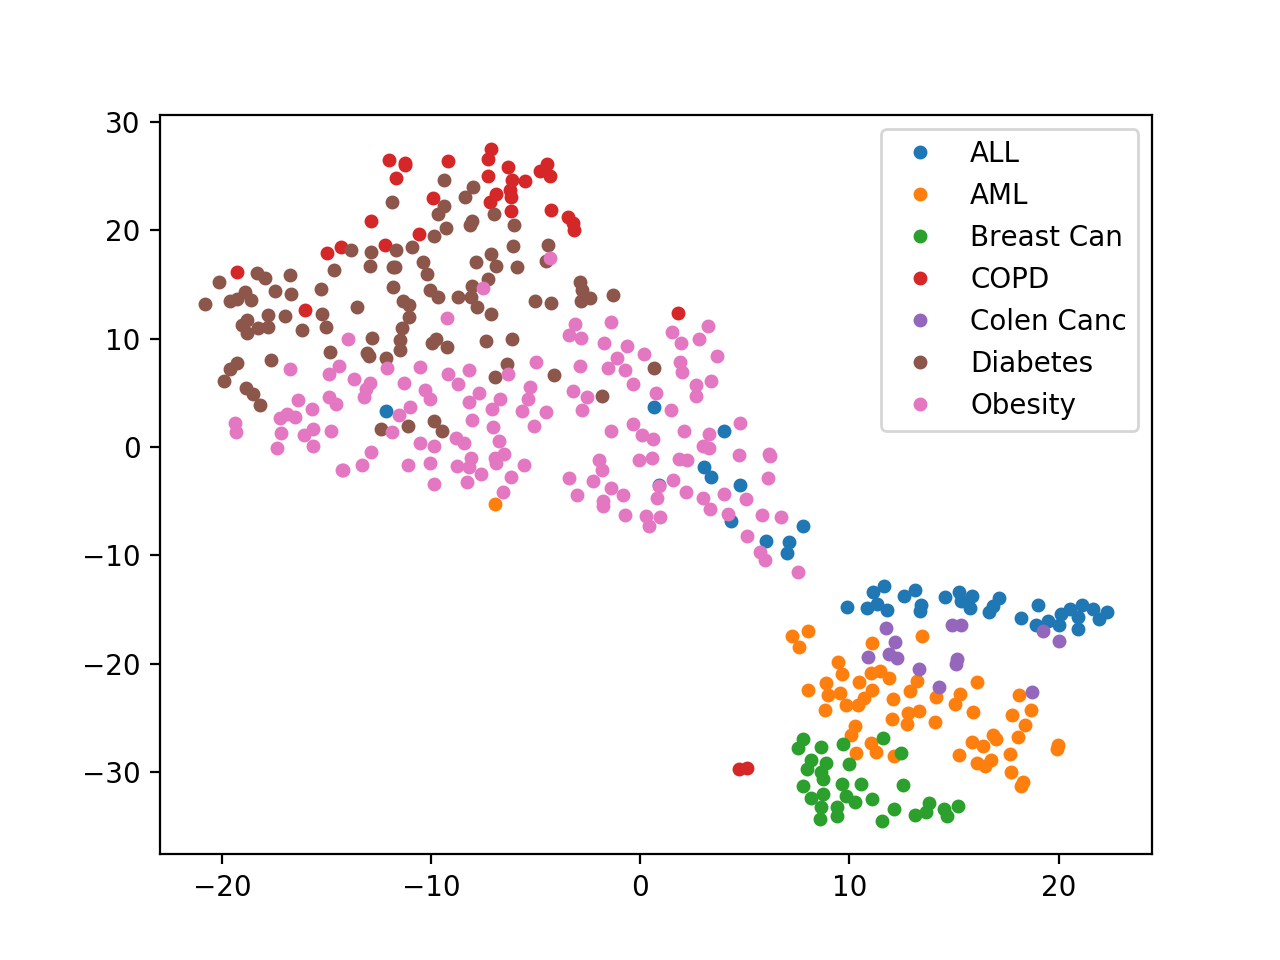
\includegraphics[width=0.7\textwidth]{tsnec.png}
		\caption{TSNE visualization of pca\_c.txt data file}
	\end{subfigure}
	\caption{(a) TSNE visualization of pca\_a.txt data file, (b) TSNE visualization of pca\_b.txt data file, (c) TSNE visualization of pca\_c.txt data file.}
	\label{fig3}
\end{figure}




\begin{figure}
	\centering
	\begin{subfigure}{1.0\textwidth}
		\centering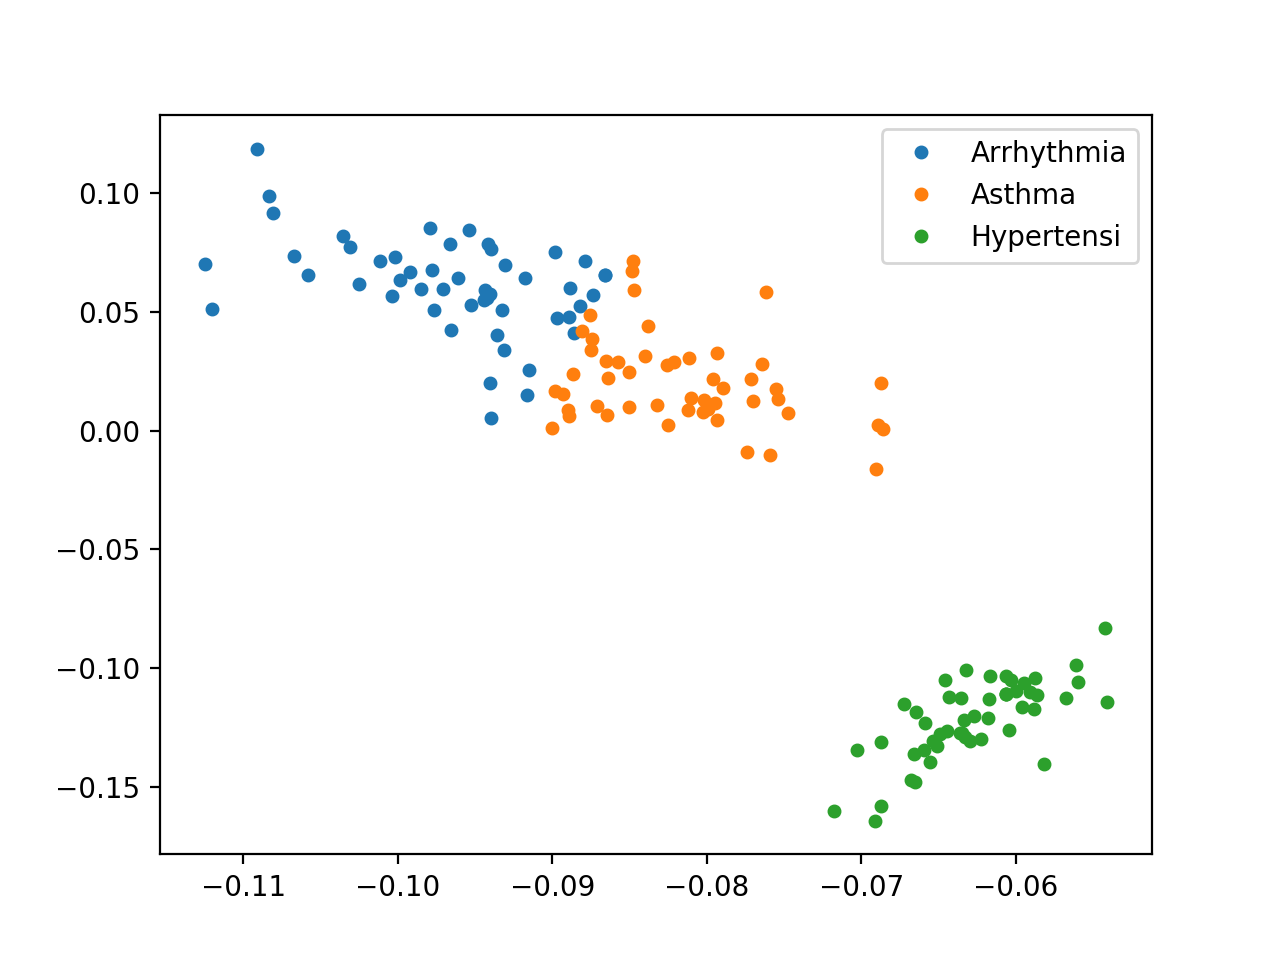
\includegraphics[width=0.7\textwidth]{svda.png}
		\caption{SVD visualization of pca\_a.txt data file}
	\end{subfigure}
	\begin{subfigure}{1.0\textwidth}
		\centering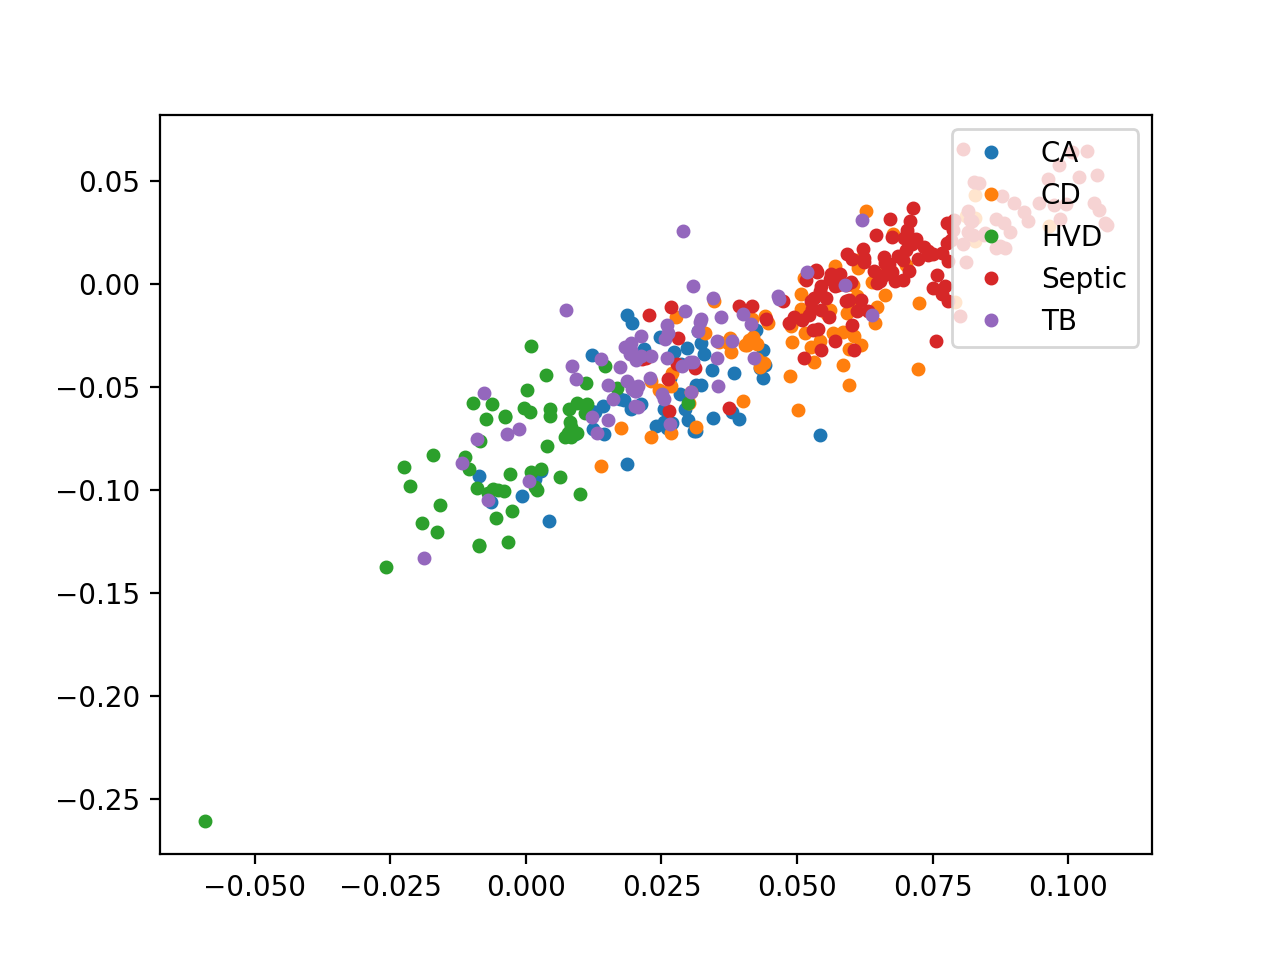
\includegraphics[width=0.7\textwidth]{svdb.png}
		\caption{SVD visualization of pca\_b.txt data file}
	\end{subfigure}
	\begin{subfigure}{1.0\textwidth}
		\centering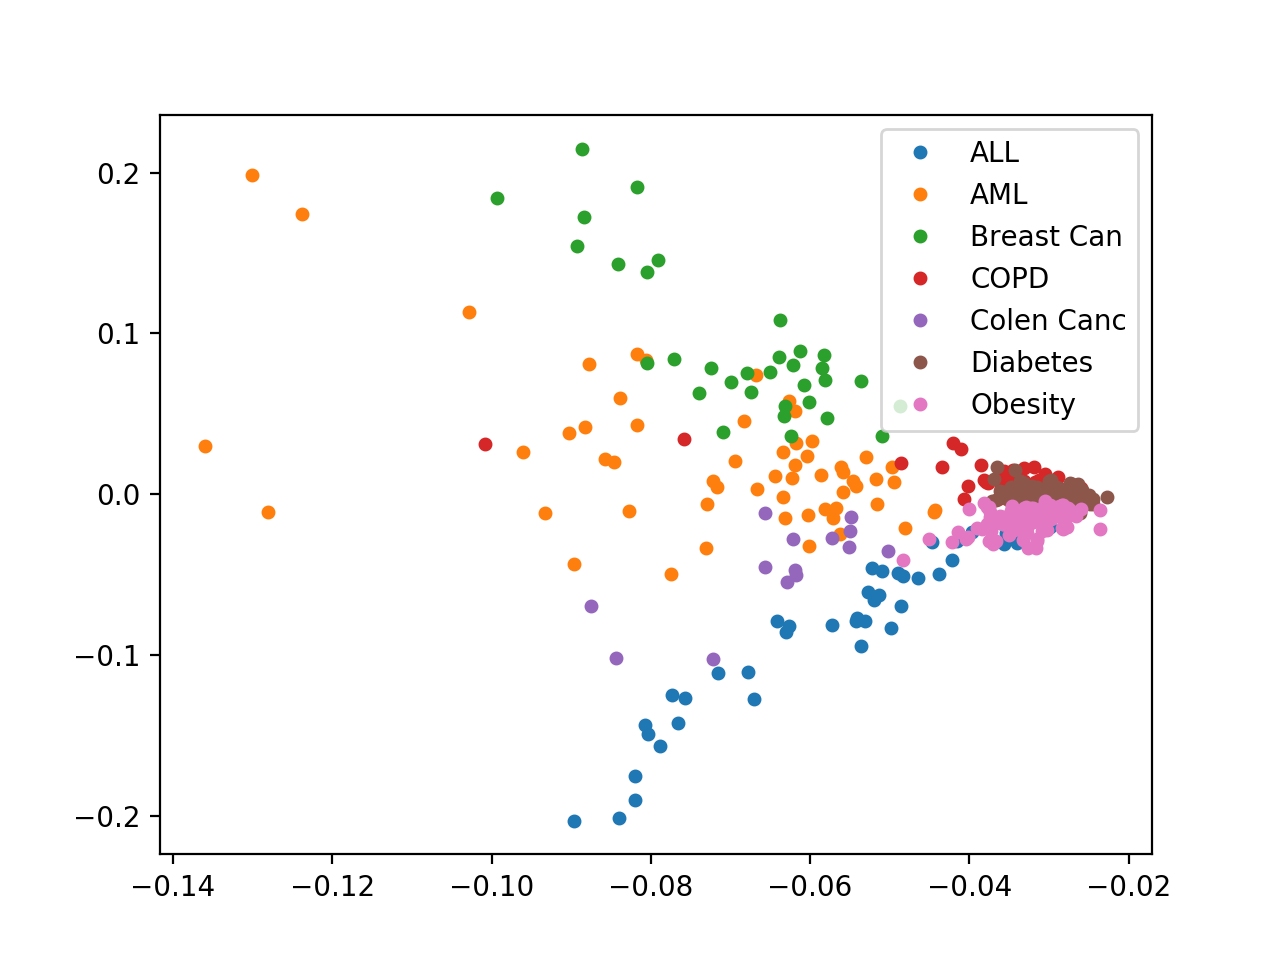
\includegraphics[width=0.7\textwidth]{svdc.png}
		\caption{SVD visualization of pca\_c.txt data file}
	\end{subfigure}
	\caption{(a) SVD visualization of pca\_a.txt data file, (b) SVD visualization of pca\_b.txt data file, (c) SVD visualization of pca\_c.txt data file.}
	\label{fig4}
\end{figure}





We can see the pca\_a data is the easiest to separate among all three dataset, as shown by the different colors denoting the different classes, the different categories of data is not overlapping with each other and is easily distinguishable. For pca\_b and pca\_c, overlapping among the different clusters exists. Taking a closer look into the result of pca\_c, we can see the clusters of data for Breast Cancer, AML and COPD are not separable in the PCA plot.

We further adopted the TSNE and SVD method to visualize the data, the result of which are shown in Figure \ref{fig3} and Figure \ref{fig4}. Comparing the result of PCA with TSNE, we can see the TSNE method is achieving similar performance as PCA in pca\_a dataset, while having better separation effect for the pca\_b and pca\_c dataset. This is in accordance with the observations of researchers in the field, as currently TSNE has become one the most widely adopted visualization methods in the field of data mining and bioinformatics.

The effectiveness of SVD is similar to PCA, which successfully separates pca\_a dataset and not effective on pca\_b dataset. The performance on pca\_c data lies in between the other two.


\subsection{Result on Apriori Algorithm} 




\bibliographystyle{splncs03}
\bibliography{PseudoBoost}




%\cleardoublepage

\end{document}
